\documentclass[11pt,a4paper]{article}
\usepackage{graphicx}
\usepackage{amsmath}
\usepackage{amssymb}
\usepackage{mathrsfs}
\usepackage{cancel}

\begin{document}
\begin{center}
\textbf{REPORTE TAREA Y PRACTICA 3-4}\\
.\\
DISEÑO DE PCB\\
\end{center}

\includegraphics[width=13cm]{upzmg.png} 
\begin{figure}[h]
\centering

\end{figure}

\begin{center}
Maria de Lourdes Gomez Islas\\
.\\
5-NOV-2019\\
Universidad Politecnica de La Zona Metropolitana de Guadalajara
\end{center}

\newpage

\section{Procedimiento del diseno}

Primero en Kitcad o en Proteus diseñamos un circuito (en este caso el de Bust) en el cual se debe obtener como funcion que el voltaje de salida sea mayor al voltaje de entrada.

\begin{figure}[h]
\centering
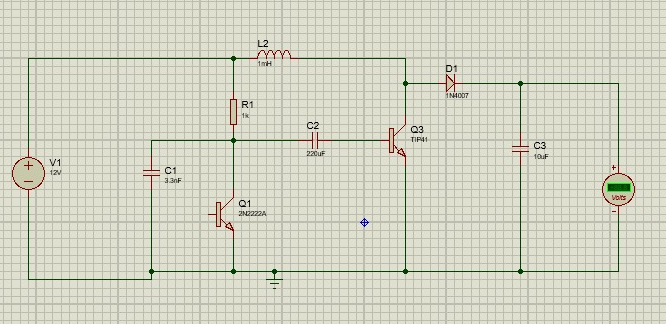
\includegraphics[width=10cm]{HTML/circuito1.png} 
\caption{Circuito en Proteus}
\end{figure}

Despues de haber hecho el circuito anterior se hara una captura de componentes en Layout teniendo como resultado la tarjeta electronica pero solo sus bases, como lo siguiente:\\

\begin{figure}[h]
\centering
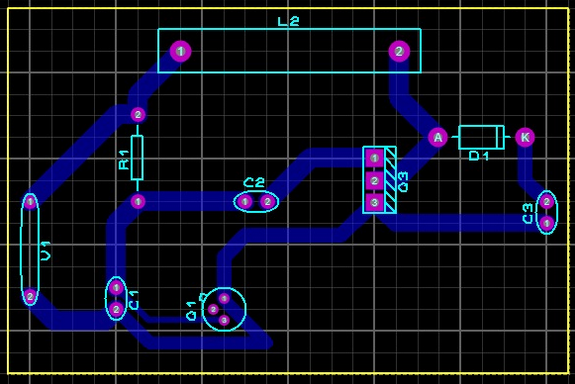
\includegraphics[width=9cm]{HTML/capturadecomponentes.png} 
\caption{Circuito en Proteus}
\end{figure}

\newpage 

Para saber como sera el circuito le damos click a la opcion de diseño 3D para asi saber si el procedimeinto es el correcto dentro de tu circuito:\\
 
\begin{figure}[h]
\centering
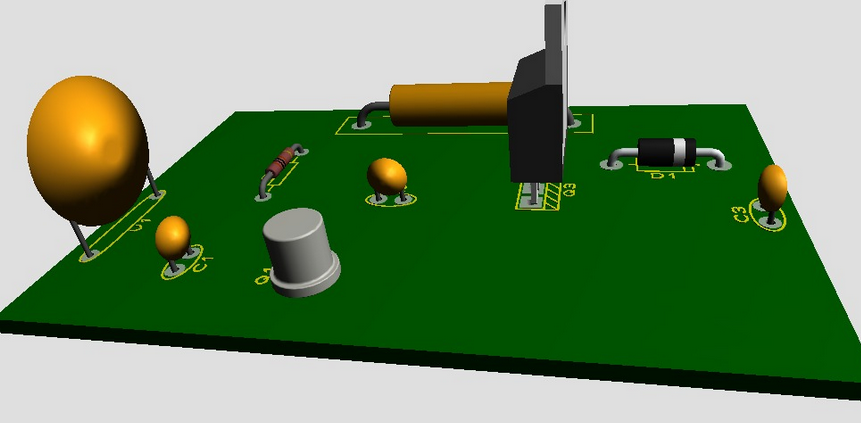
\includegraphics[width=8cm]{HTML/diseño3D.png} 
\caption{Circuito en Proteus}
\end{figure}

Nos dimos cuenta que en el circuito las celdas no estaban rellenas:\\

\begin{figure}[h]
\centering
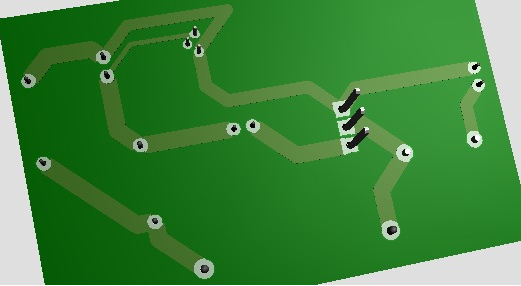
\includegraphics[width=9cm]{HTML/simulacion3D.png} 
\caption{Circuito en Proteus}
\end{figure}

\newpage 

Antes debemos que tener en cuenta que el circuito es erroneo si las pistas son de 90grados, es decir, cuando una pista esta completamente inclinada los electrones no podran conducir de manera correcta a que si la pista la colocamos a un grado de 45. Bueno siguiendo despues de la sujerencia continuamos con el relleno el cual nos resulto de la siguiente forma:\\

\begin{figure}[h]
\centering
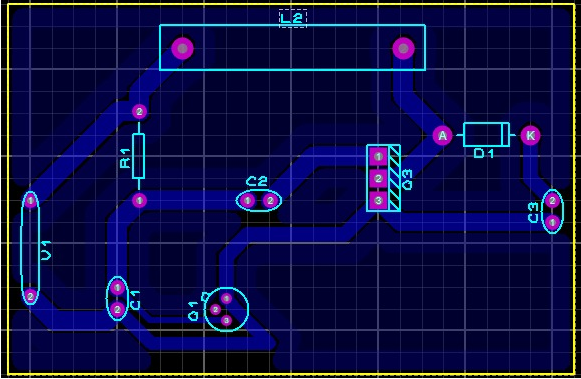
\includegraphics[width=9cm]{HTML/relleno.png} 	
\caption{Circuito en Proteus}
\end{figure}

\begin{figure}[h]
\centering
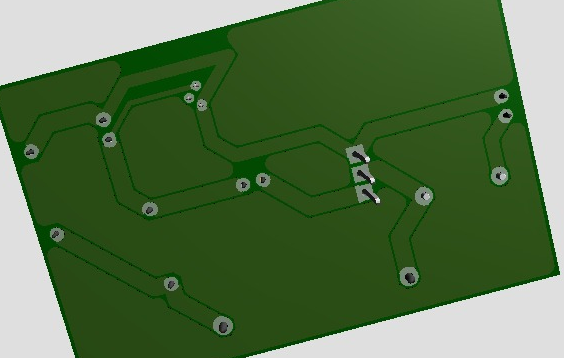
\includegraphics[width=9cm]{HTML/relleno3D.png} 
\caption{Circuito en Proteus}
\end{figure}

\newpage 

Despues de haber terminado con el circuito y de haber corregido errores, lo comprimimos en la opcion \textbf{windows PDF}, quitamos todas las opciones a excepcion de la \textbf{Bottom Lane} y \textbf{Aceptar}, esta opcion nos sirve para que al momento de imprimir se vean solo las celdas y asi planchar en la baquelita, el resultado es el siguiente:\\

\begin{figure}[h]
\centering
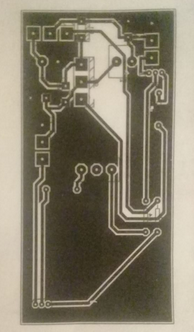
\includegraphics[width=5cm]{HTML/Impresion.png} 
\caption{Circuito en Proteus}
\end{figure}

\section{Conclusion}
Al momento de hacer el planchado se tubo complicaciones, lo cual lo recomendado seria hacerlo en una hoja delgada, con papel contac para ser exactos y esperar de 10 a 15 minutos.


\end{document} 